\documentclass{article}


\usepackage{arxiv}

\usepackage[utf8]{inputenc} % allow utf-8 input
\usepackage[T1]{fontenc}    % use 8-bit T1 fonts
\usepackage{hyperref}       % hyperlinks
\usepackage{url}            % simple URL typesetting
\usepackage{booktabs}       % professional-quality tables
\usepackage{amsfonts}       % blackboard math symbols
\usepackage{nicefrac}       % compact symbols for 1/2, etc.
\usepackage{microtype}      % microtypography
\usepackage{lipsum}
\usepackage{graphicx}
\usepackage{subfigure}
\graphicspath{ {./images/} }


\title{k-NN Sampling for Visualization of Dynamic Data Using LION-tSNE - analysis}


\author{
 Gędłek Paweł \\
  Wydział Informatyki, Elektroniki i Telekomunikacji\\
  Akademia Górniczo-Hutnicza \\
  Kraków \\
  \texttt{gedlek@student.agh.edu.pl} \\
  \And
Wójtowicz Patryk \\
  Wydział Informatyki, Elektroniki i Telekomunikacji\\
  Akademia Górniczo-Hutnicza \\
  Kraków \\
  \texttt{wojtowicz@student.agh.edu.pl} \\
}


\begin{document}
\maketitle
\begin{abstract}

Obecnie rośnie zapotrzebowanie na metody wizualizacji dynamicznie zmieniających się dużych zbiorów danych. Taka potrzeba pojawia się między innymi w medycynie, gdy aktualne dane (np. stan pacjenta) zmienia się na bieżąco. Co za tym idzie istotnym elementem analizy danych, jest nie tylko dobór odpowiedniej metody wizualizacji, ale także sposobu próbkowania. W niniejszym raporcie prezentujemy analizę oraz wizualizację danych opartą na metodzie Local Interpolation with Outlier coNtrol t-distributed stochastic neighbor embedding (LION tSNE) wraz z wykorzystaniem idei kNN samplingu. Jako próbę kontrolną metody LION tSNE użyliśmy metody tSNE, a także losowo wybranych próbek oraz selektywnie wybranych próbek metodą k najbliższych sąsiadów. Testy zostały przeprowadzone na czterech różnych datasetach oraz wydajność metod została zmierzona z użyciem wiarygodnej metryki.

\end{abstract}


% keywords can be removed
% keywords{First keyword \and Second keyword \and More}

\tableofcontents

\section{Metoda tSNE}
\label{sec:tSNE}
\paragraph{}
\subsection{Czym właściwie jest tSNE?}
Algorytm tSNE(t-Distributed Stochastic Neighbor Embedding) którego autorami są Laurens van der Maaten oraz Geoffrey Hinton bazuje na metodzie SNE, której głównym założeniem jest reprezentacja wielowymiarowych danych w możliwy do zobrazowania dla człowieka dwu- lub trzy-wymiarowej przestrzeni. Osiąga się to poprzez modelowanie wysoko wymiarowych obiektów poprzez dwu- lub trzy-wymiarowe punkty w taki sposób, że zbliżone obiekty modelowane są poprzez bliskie sobie punkty, a oddalone obiekty modelowane są poprzez oddalone od siebie punkty z dużym prawdopodobieństwem. 
        
\subsection{Algorytm tSNE - podstawy matematyczne}
Algorytm tSNE w dużym uproszczeniu sprowadza się do następujących kroków:
\begin{itemize}
	\item Algorytm tSNE konwertuje odległości między parami punktów w funkcję rozkładu prawdopodobieństwa określająca podobieństwo pomiędzy parami punktów.  
	\item Rozbieżność między podobieństwem wysoko wymiarowych danych z nisko-wymiarowymi danymi jest mierzona poprzez dywergencje Kullbacka-Leiblera i minimalizowana metodą gradientową poszukiwania minimum lokalnego
\end{itemize}

Mamy dany zbiór wejściowy $X = \{x_1, x_2 ... x_n\}$  gdzie dla każdego $x_i \in \mathbb{R}^{D} $ jest D-wymiarowym wektorem. Zbiór ten zostanie przekształcony do postaci $Y = \{y_1, y_2 ... y_n\}$  gdzie każde $y_i \in \mathbb{R}^{d} $ jest d-wymiarowym wektorem oraz $ d \ll D $ (zazwyczaj d = 2 lub 3). Podobieństwo pomiędzy parą punktów wejściowych $ x_i $ oraz $ x_j $ oznaczamy poprzez $ p_{j/i} $, które jest prawdopodobieństwem wybrania $ x_j $ jako sąsiada $ x_i $ według funkcji gęstości prawdopodobieństwa na rozkładzie normalnym gdzie $ x_i $ stanowi centrum.  $ p_{j/i} $ definiujemy jako:
\[
     p_{j|i} = \frac{exp(\frac{-d(x_i,x_j)^{2})}{2\sigma_i^{2}})}{\sum_{k \neq i}^{n} exp(\frac{-d(x_i,x_k)^{2})}{2\sigma_i^{2}}))} \quad p_{i|i} = 0  \quad p_{ij} = \frac{p_{j|i}+p_{i|j}}{2n} 
\]

gdzie: \\
$d(x_i,x_j)$ - odległość pomiędzy punktami $x_i$ oraz $x_j$ w oryginalnym wymiarze\\
$\sigma_i$ - wariancja dla punktu $x_i$

Aby orzymać zbiór wyjściowy Y, losujemy $n$ punktów w docelowym wymiarze i dla każdego z nich wyznaczamy podobną funkcję gęstości prawdopodobieństwa (tym razem jest to rozkład Studenta):

\[
     q_{ij} = \frac{(1+d(y_i,y_j)^{2})^{-1}} {\sum_{k \neq l}^{n}((1+d(y_k,y_l)^{2})^{-1})}
\]
gdzie: \\
$d(y_i,y_j)$ - odległość pomiędzy punktami $y_i$ oraz $y_j$ w docelowym wymiarze\\

W ten sposób otrzymujemy łączone rozkłady gęstości prawdopodobieństwa P i Q dla wszystkich punktów ze zbiorów odpowiednio X i Y. Podobieństwo między nimi (a właściwie dowolnymi 2 rozkładami) określa dywergencja Kullbacka-Leiblera:

 \[
     C = KLDIV(P||Q) = \sum_i^n \sum_j^n p_{ij} log \frac{p_{ij}}{q_{ij}}
\]
która staje się naszą funkcją kosztu, którą chcemy zminimalizować, robi się to algorytmem spadku po gradiencie (\textit{Gradient Descent}). Pochodna cząstkowa C dla $y_{i}$ to:
\[
     \frac{\delta C}{\delta y_i} = 4 \sum_j^n (p_{ij} - q_{ij})(y_i - y_j)(1 + d(y_i - y_j)^2))^{-1}
\]

\subsection{Sposób wyboru wariancji}

Wariancję $\sigma_i$ dla punktu $x_i$ wybiera się na podstawie parametru algorytmu ustawianego przez użytkownika zwanego \textit{Perplexity}. Definjujemy:
\[
    Perp(i) = 2^{H(P_i)} \quad H(P_i) = \sum_j p_{j|i} log(\frac{1}{p_{j|i}})
\]

gdzie: \\
$H(P_i)$ - entropia Shannona dla zmiennej losowej $P_i$

Dla rozkładu normalnego im większa entropia, tym większa wariancja, tym "grubsze ogony" funkcji dzwonowej, tym większe prawdopodobieństwo wybrania bardziej odległych sąsiadów punktu $x_i$. Zazwyczaj dla wszystkich punktów $Perp(i)$ ustawiane jest na taką samą wartość $p$. Im mniej "gęsty" jest nasz zbiór danych tym $Perp$ powinno być większe.

\subsection{Workflow metody tSNE}

\begin{figure}[h]
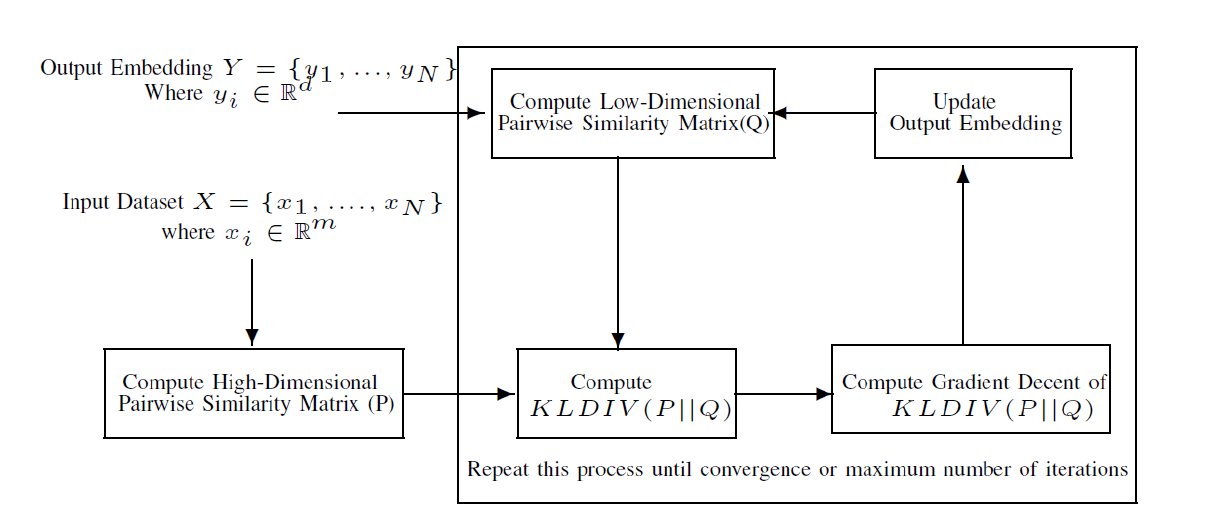
\includegraphics[scale=0.52]{algorithm_TSNE.PNG}
\caption{Algorytm tSNE - workflow modelu}
\end{figure}

\subsection{Pseudokod metody tSNE}

\begin{figure}[h]
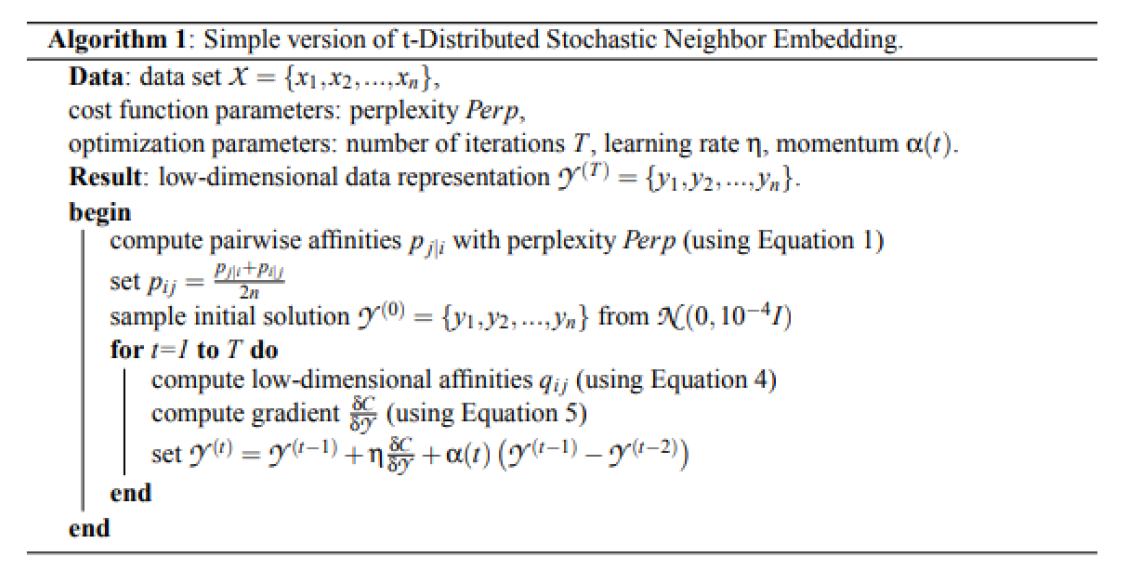
\includegraphics[scale=0.52]{algorithm_TSNE_pseudocode.PNG}
\caption{Algorytm tSNE - pseudokod}
\end{figure}

\section{Metoda LION tSNE}
\label{sec:lionTSNE}
\paragraph{}
Algorytm t-SNE nie odpowiada na pytanie jak dodawać nowe dane (lub wizualizować dynamiczne zmiany danych) do utworzonego modelu. Z pomocą przychodzi metoda     LION tSNE (Local Interpolation with Outlier coNtrol t-Distributed Stochastic Neighbor Embedding). Korzysta ona z 2 metod dodawania nowych punktów: 
\begin{itemize}
    \item Dla inlierów czyli punktów które mogą potencjalnie należeć do jakiegoś klastra - Inverse Distance Weight Interpolation (IDW)
    \item Dla outlierów specjalna heurystyka (Outlier Placement) oszacowania ich pozycji na wizualizacji zapewniająca odpowiednią odległość od innych punktów
\end{itemize}

\subsection{Pseudokod metody LION tSNE}
Z oryginalnego datasetu wybierane są \textbf{losowo} punkty i na ich podstawie tworzone jest mapowanie do niższego wymiaru (za pomoca standardowego algorytmu t-SNE). Następnie:

\begin{figure}[h]
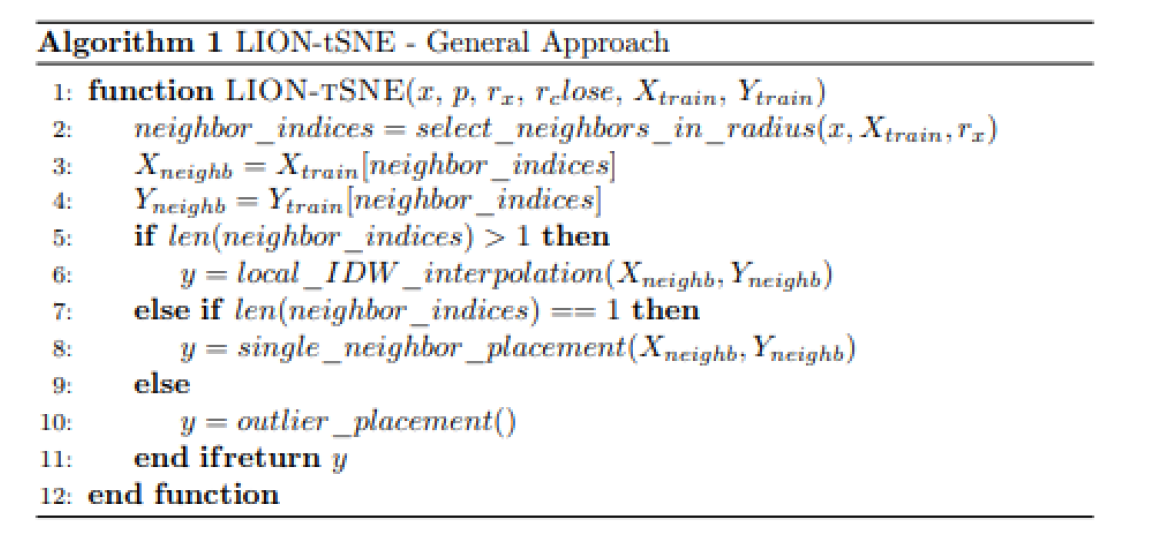
\includegraphics[scale=0.52]{algorithm_lionTSNE_pseudocode.PNG}
\caption{Algorytm tSNE - pseudokod}
\end{figure}

\subsection{LION tSNE - IDW}

Gdy algorytm zadecyduje, że dany punkt jest inlierem, stosowana jest technika Inverse Distance Weight Interpolation (IDW). Dla nowego punktu  $x$ jego pozycja F(x) w nowym wymiarze jest wyliczana następująco:
\[
    F(x) = \sum_{d(x - x_i) \leq r_x} w_i(x) y_i, gdzie \quad w_i(x) = \frac{d(x - x_i)^{-p}}{\sum_{d(x - x_j) \leq r_x} d(x - x_j)^{-p}}
\]
$r_x$ - promień odległości dla lokalnego sąsiedztwa w którym jest dodawany nowy punkt, parametr wywołania \\
$p$ - parametr wywołania

Zauważmy, że gdy $ x \rightarrow x_i$ to $d(x - x_i)^{-p} \rightarrow \infty $ i $w_i(x) \rightarrow 1$ i $F(x) \rightarrow y_i$

\subsection{LION tSNE - outlier placement}

Główną ideą outlier placementu jest następująca: jeśli x jest outlierem to 
odpowiadająca jej po zmapowaniu wartość y powinna także być zwizualizowana 
jako outlier. Aby odnaleźć takie wartości, musimy znaleźć położenie y, takie 
że nie ma żadnych sąsiadów w promieniu $r_y$. 
Promień $r_y$ jest jednym z parametrów algorytmu i jeśli zostanie wybrana
zbyt duża wartość, wtedy z racji na duże odległości między punktami, zmniejsza 
się czytelność wykresu natomiast jeśli promień zostanie wybrany zbyt mały klastry 
i wartości odstające mogą być nierozróżnialne. Dlatego też wartość $r_y$ może 
być wyznaczona na podstawie pewnego percentylu rozkładu odległości najbliższych 
sąsiadów w przestrzeni y (np. 95-ty lub 99-ty percentyl).

\section{kNN sampling}
\label{sec:kNN}

\subsection{kNN sampling w LION tSNE}

Autorzy artykułu zasugerowali, że sposób próbkowania danych zastosowany w tSNE jest niewystarczający chociażby przy dynamicznie zmieniających się danych. Jednocześnie przedstawili kilka kroków potrzebnych do zrealizowania idei k-NN samplingu.
\begin{enumerate}
    \item Czyszczenie danych za pomocą eliminacji redundantnych punktów i zainicjalizowanie pustych zmiennych odpowiednimi wartościami.
    \item Dobór właściwego zbioru treningowego poprzez k-NN sampling.
    \item Rzutowanie zbioru treningowego na nisko wymiarową przestrzeń oraz dodanie nowych punktów do modelu tSNE.
    \item Dla nowych danych interpolacja ich do istniejącego modelu za pomocą LION-tSNE
    \item Wyliczenie precyzji k-NN samplingu dla całego zbioru danych.

\end{enumerate}

\subsection{Wybór zbioru treningowego poprzez k-NN sampling}

Zaproponowana idea k-NN samplingu opiera się na wyliczeniu Nearest Neighbor score (NNscore)
oraz Mutual Nearest Neighbor score (MNNscore). Mamy dany graf skierowany $G=(V, E)$, gdzie 
krawędź $E(v_1, v_2)$ oznacza, że $v_2$ jest sąsiadem $v_1$, natomiast sąsiedztwo $v_1$ oznaczamy jako $N_{v1}$. Stopień wychodzący każdego wierzchołka jest równy k, a stopień wchodzący zależy od wartości współczynnika sąsiedztwa innych wierzchołków. W celu wyznaczenia optymalnego zbioru treningowego dobieramy odpowiednie k oraz zbiór punktów wejściowych mapujemy na wierzchołki grafu k-NN.

Wyznaczamy NN\_score, który odpowiada stopniu wchodzącemu wierzchołka $x_i$:

\[NNscore(x_i) = | \{x_j | x_i \in N_{x_{j}} \} |. \forall_{j \neq i}x_j \in X \]

Gdzie X jest zbiorem danych wejściowych a $ N_{x_{j}} $ sąsiedztwem $ x_j $
Następnie wyliczamy MNNscore, który dla $x_i$ jest równy conajwyżej k:

\[MNNscore(x_i) = | \{x_j | x_i \in N_{x_{j}} \land x_i | x_j \in N_{x_{i}} \} |. \forall_{j \neq i}x_j \in X \]

Ostatecznie dobór punktu $x_i$ jako próbki treningowej oraz jego sąsiedztwo jest dany jako: 
\[ train\_sample = first\_index\{argmax_{x_{i} \in X} \{ NNscore(x_i) \} \cap argmax_{x_{i} \in X} \{ MNNscore(x_i) \} \} \]

\subsection{Dodanie nowych punktów do modelu tSNE}

W LION-tSNE stosujemy IDW i Outlier Placement. 
Nowe dane mogą być dodawane do modelu tSNE na dwa sposoby, na podstawie 
wyliczonych parametrów $r_{xNN}, r_{yNN}$ oraz $r_{close}$. Wartość $r_{xNN}$ 
oznacza minimalny promień zbioru wejściowego, co z pomocą pewnej heurystyki 
pozwala na wskazanie czy dany punkt jest wartością właściwą czy odstającą.
Parametr $r_{close}$ pozwala na zidentyfikowanie próbek odstających powiązanych 
z wartościami odstającymi znajdującymi się w modelu tSNE.
Natomiast $r_{yNN}$ wyznacza minimalną odległość pomiędzy punktami ze zbioru wejściowego, 
a próbkami odstającymi oraz dla wartości odstających pomiędzy nimi.

\subsection{Wyliczenie precyzji k-NN samplingu}

Nowo dodane próbki są umieszczane pośród próbek treningowych o podobnej charakterystyce. 
Aby to zbadać, dla każdej nowo dodanej próbki, wyliczany jest stopień precyzji oraz obserwowany
jest procent k sąsiadów o podobnej charakterystyce. Precyzja k-NN zazwyczaj zależy od 
parametru k, który jest zwykle ustawiony na stałe. Mała wartość k oznacza dobrą precyzje, 
natomiast jeśli wartość k zaczyna rosnąć to wtedy precyzja maleje. Dlatego też odpowiedni dobór
k stanowi ważny element k-NN samplingu.

\section{Wyniki projektu}
\label{sec:results}
\paragraph{}
W pierwszej części projektu zdecydowaliśmy się na analizę działania metody LION tSNE i
zwracanych przez nią rezultatów. Ważnym elementem okazało się sprawdzenie
jaki wpływ na wizualizację ma odpowiednie próbkowanie danych wejściowych. Serię
eksperymentów przeprowadziliśmy na zbiorach IRIS \cite{iris-dataset} oraz MNIST \cite{mnist-dataset}, a jako próbkę kontrolną
wybraliśmy tradycyjne tSNE. W połowie eksperymentów mieliśmy do czynienia z losowo
wybranym zbiorem testowym natomiast w drugiej połowie posłużyliśmy kNN
samplingiem będącym jedną z części naszego projektu. W dalszej fazie eksperymentów posłużyliśmy się nieco bardziej złożonymi zbiorami danych, a mianowicie Fashion MNIST \cite{fmnist-dataset} oraz Reuters  \cite{reuters-dataset}. 

\paragraph{}
Spróbujmy odpowiedziec na pytanie dlaczego odpowiednie próbkowanie danych jest takie ważne?
Losowe próbkowanie polega na pseudolosowym doborze rekordów z wybranego
datasetu, co jest obarczone możliwością wyboru nierównych podzbiorów danych klas oraz
ryzykiem dużego stopnia wariancji danych.

\begin{figure}[h]
\hfill
\subfigure[losowe próbkowanie]{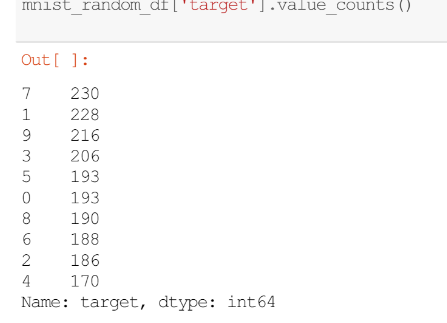
\includegraphics[scale=0.62]{mnist-random-sampling.PNG}}
\hfill
\subfigure[próbkowania k najbliższych sąsiadów]{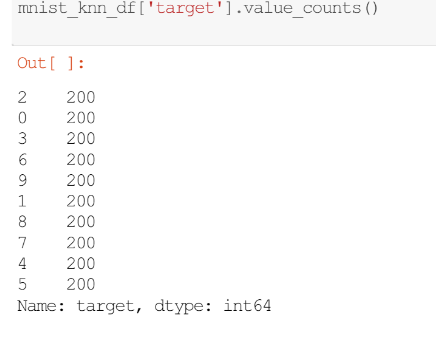
\includegraphics[scale=0.62]{mnist-knn-sampling.PNG}}
\hfill
\caption{Podział na poszczególne klasy dla zbioru MNIST}
\end{figure}

W przypadku przeprowadzonego przez nas kNN samplingu, zauważyliśmy, że zwraca dość obiecujące wyniki, a mianowicie polega na tym, że wyliczamy za pomocą Nearest Centroid Classifier (pochodzącego z biblioteki scikit-learn) centroidy dla poszczególnych klas. Następnie dla każdej klasy wyszukujemy k najbliższych sąsiadów centroida klasy i umieszczamy je w zbiorze testowym. Tak przeprowadzone próbkowanie rozwiązuje oba problemy wspomniane powyżej (występujące w losowym próbkowaniu).

\subsection{Przeprowadzone eksperymenty}
\paragraph{}
Poszczególne wizualizacje przedstawione poniżej zostały uporządkowane w nastęopujący sposób:
górny wiersz - losowy sampling, dolny wiersz - knn sampling, a także odpowiednio od lewej tSNE, LION tSNE, PCA + LION tSNE, MDS + LION tSNE.  

\paragraph{}
\begin{itemize}
    \item IRIS Dataset \cite{iris-dataset}
    \paragraph{}
    Jest to stosunkowo mały zbiór zawierający opisy czterech własności, trzech różnych
    gatunków irysów. Z racji na niewielki rozmiar, zbiór okazał się przydatny do testowania
    samplingu danych (wybieraliśmy 120 spośród 150 dostępnych rekordów), jednak wydaję
    się zbyt mały dla niektórych metod, aby stworzyć w pełni wiarygodny model.
    
    
\begin{figure}[h]
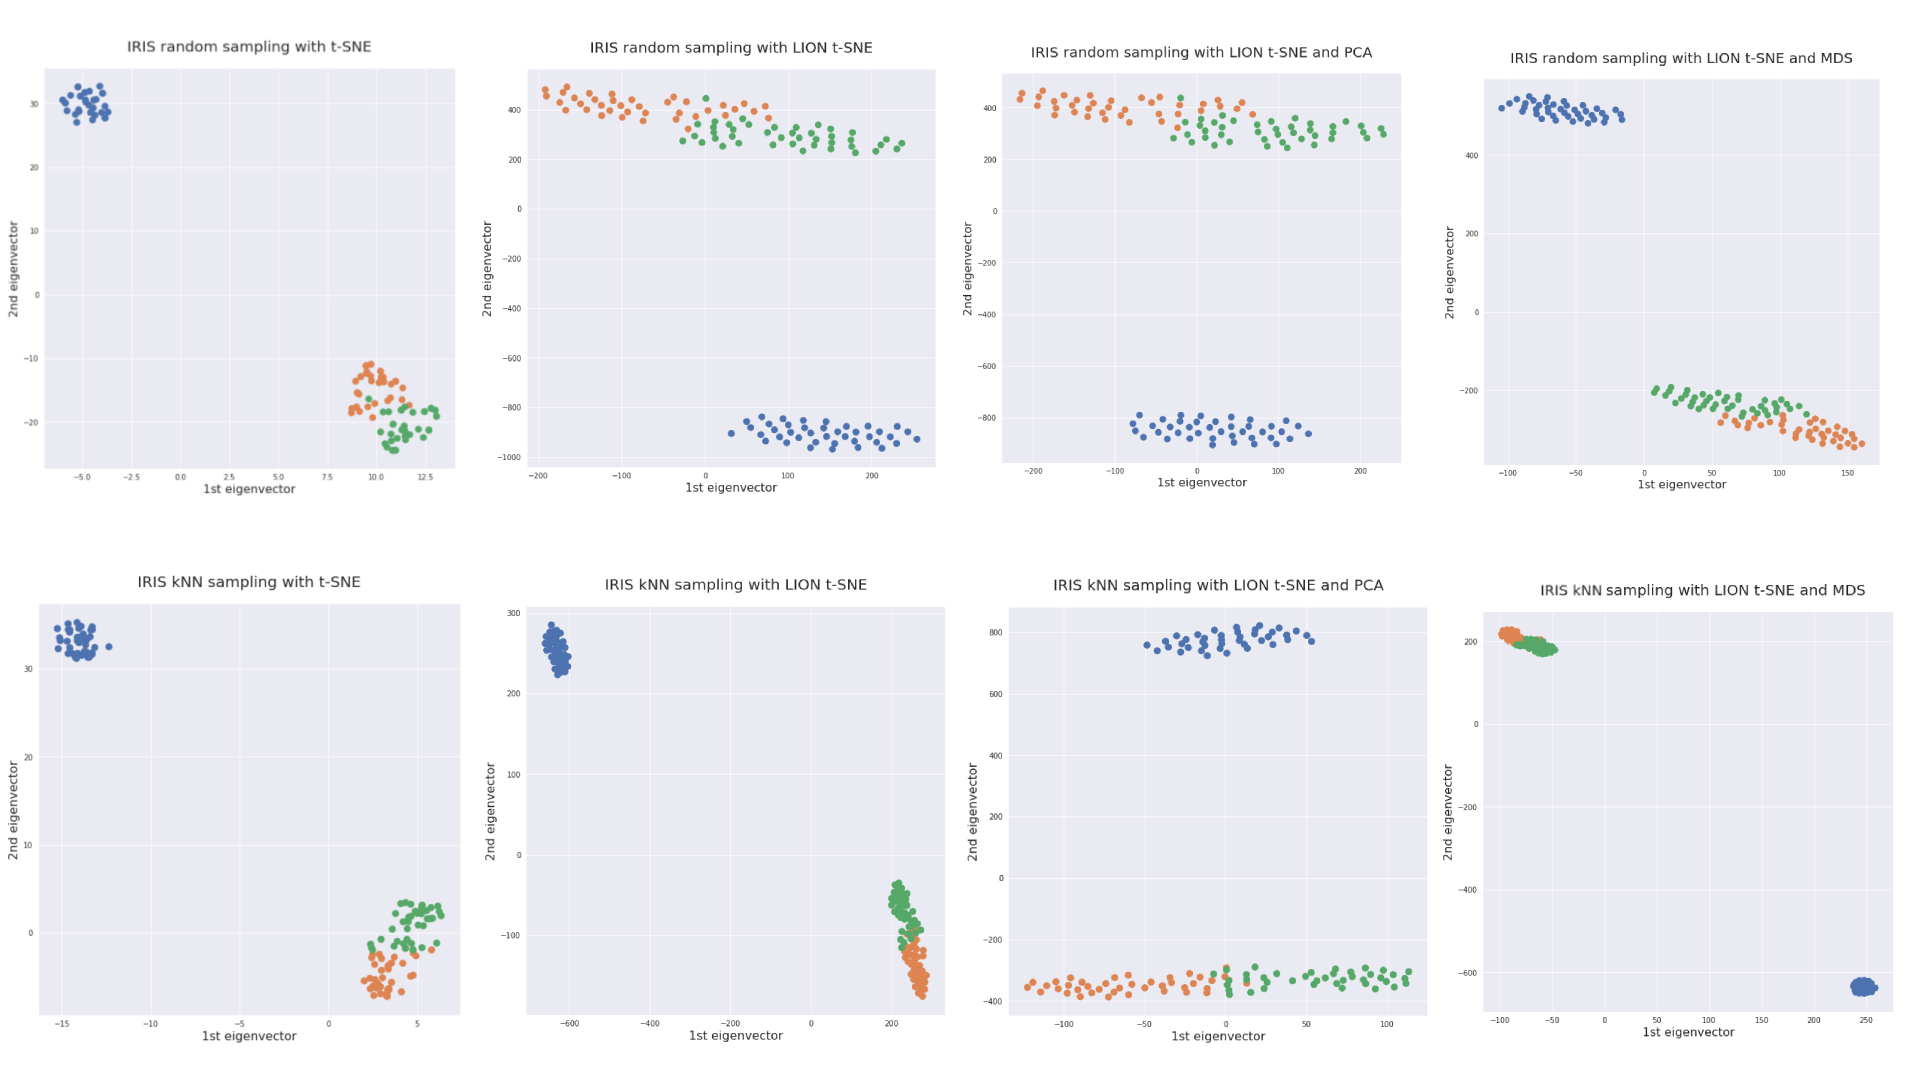
\includegraphics[scale=0.25]{iris-dataset-results.png}
\caption{Wizualizacja IRIS Dataset za pomocą różnych metod}
\end{figure}
    
    \item MNIST Dataset \cite{mnist-dataset}
    \paragraph{}
    Dataset zawierający opisy cyfr pisanych reprezentowanych jako obrazki 28x28 pikseli. W
    przypadku eksperymentów na tym zbiorze danych posłużyliśmy zbiorem testowym
    zawierającym 2000 rekordów (mniej więcej 200 obrazków na daną klasę).


\begin{figure}[h]
\begin{center}
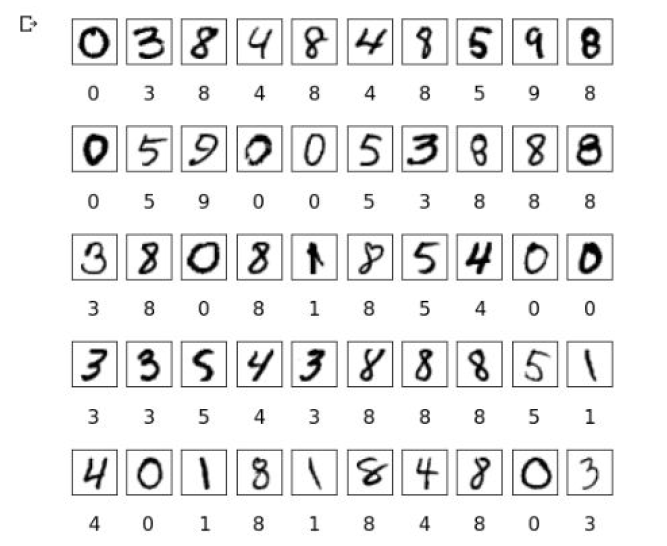
\includegraphics[scale=0.5]{mnist-visualisation.PNG}
\caption{Wizualizacja przykładowych danych ze zbioru MNIST}
\end{center}
\end{figure}

\begin{figure}[h]
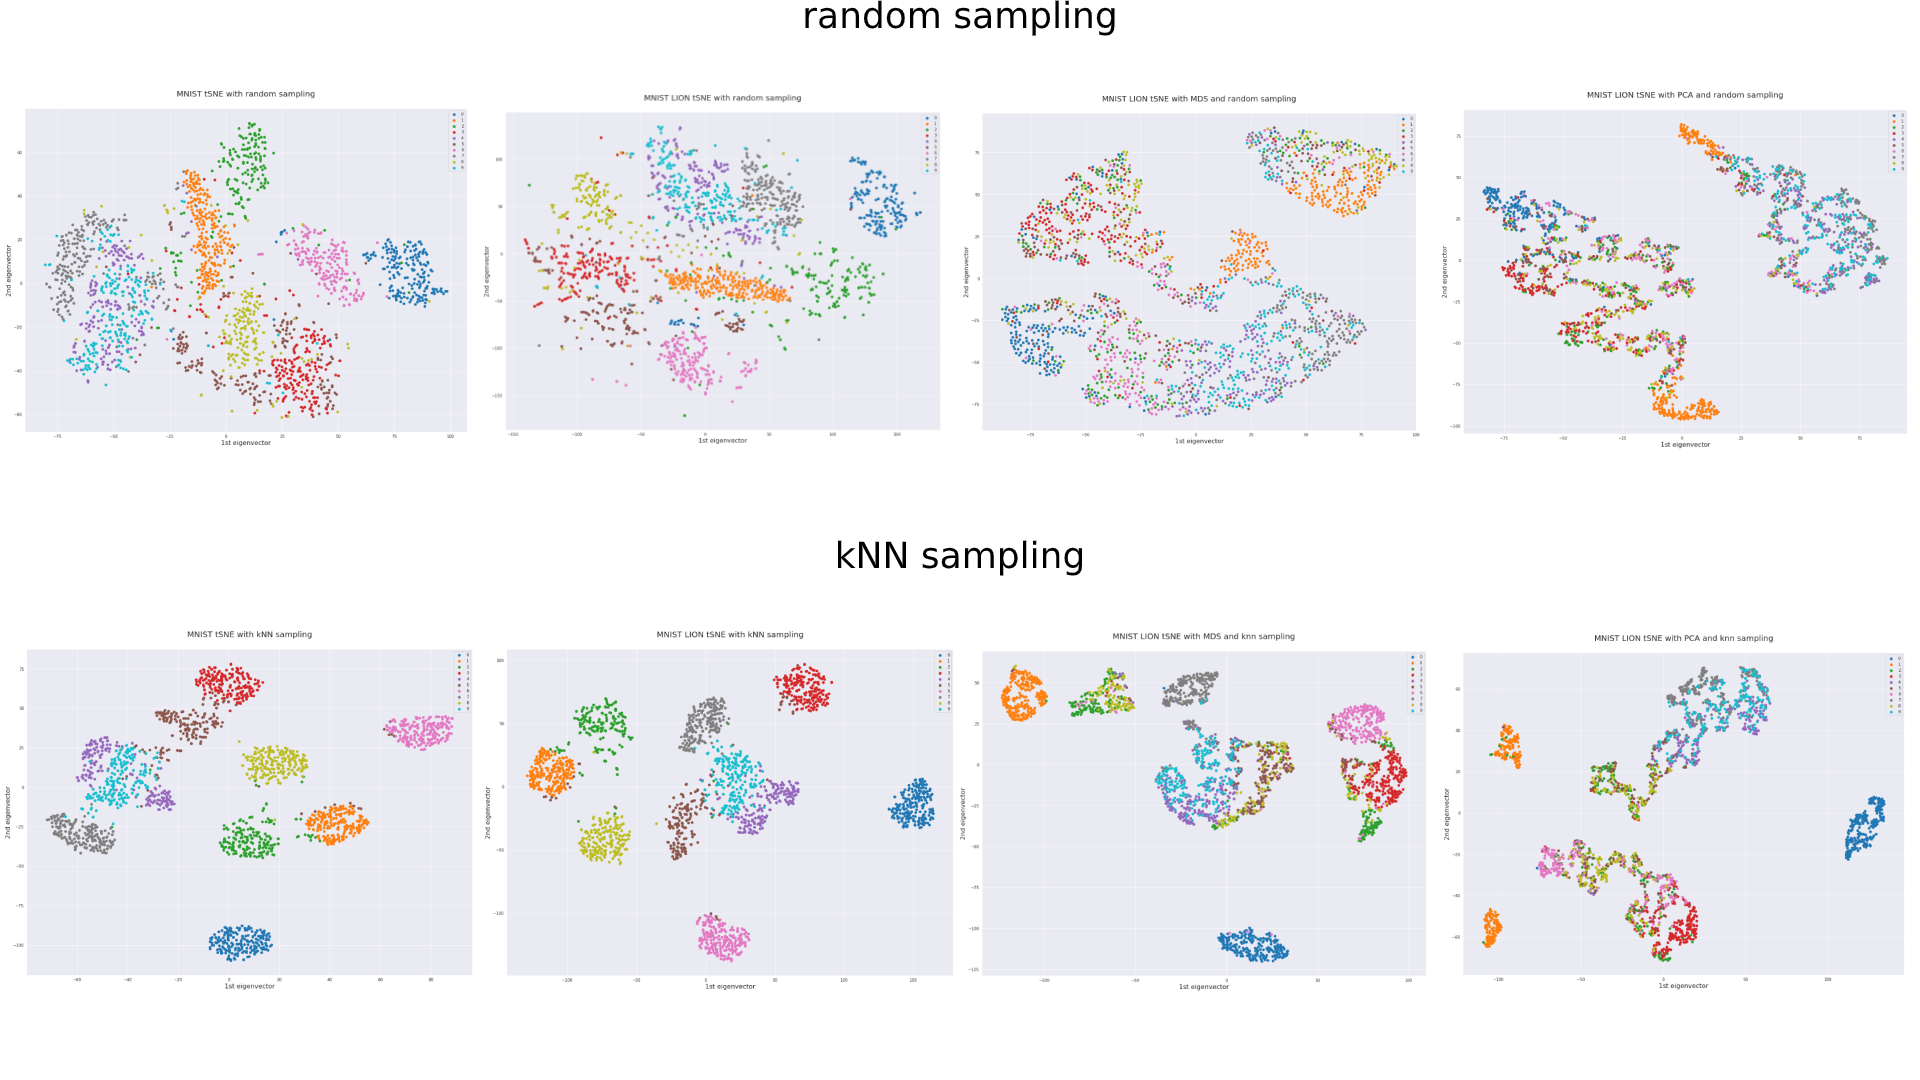
\includegraphics[scale=0.25]{mnist-dataset-results.png}
\caption{Wizualizacja MNIST Dataset za pomocą różnych metod}
\end{figure}

    \item Fashion MNIST Dataset \cite{fmnist-dataset}
    \paragraph{}
    Zbiór danych Fashion MNIST zawiera tysiące zdjęć ubrań pochądzących z zasobów sklepu Zalando. Każde zdjęcie zostało przekonwertowane na macierz 28x28 pikseli, w której wartości są z przedziału 0-255, co odpowiada skali szarości tych obrazków. Co więcej, mamy tu do czynienia z 10 różnymi rodzajami ubrań, a mianowicie: 
    
    \begin{enumerate}
        \item T-shirt/top
        \item	Trouser
        \item	Pullover
        \item	Dress
        \item	Coat
        \item	Sandal
        \item	Shirt
        \item	Sneaker
        \item	Bag
        \item	Ankle boo
    \end{enumerate}
    \paragraph{}
    Zatem zbiór ten wzoruję się częsciowo na zbiorze MNIST jednak jest zdecydowanie bardziej skomplikowany, co jest niejednokrotnie pożądane w niektórych zadaniach związanych z uczeniem maszynowym. Oto kilka przykładowych zdjęć z tego zbioru:
    
\begin{figure}[h]
\begin{center}
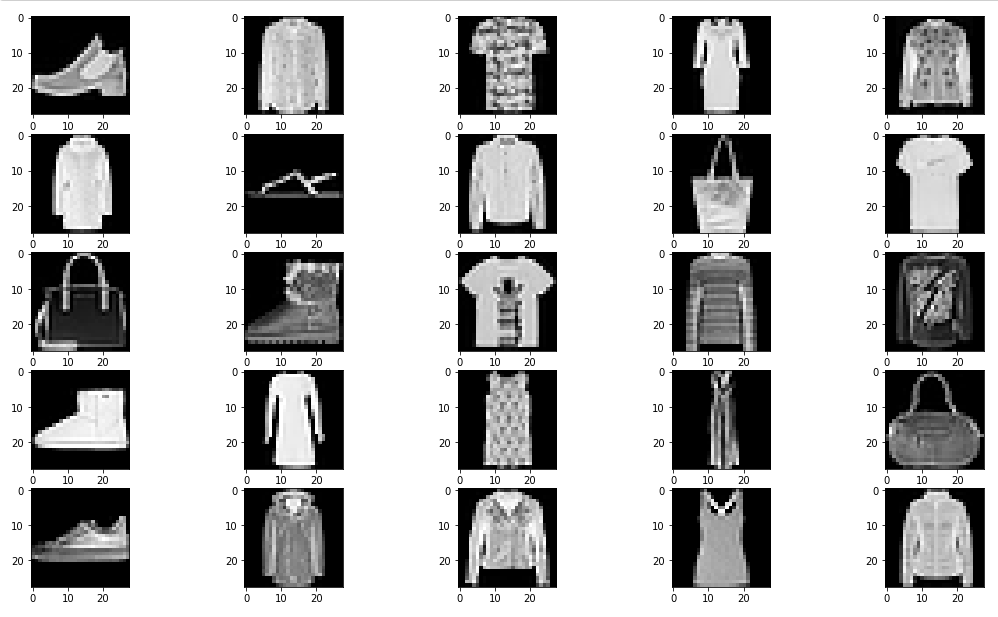
\includegraphics[scale=0.45]{fmnist-visualisation.PNG}
\caption{Wizualizacja przykładowych danych ze zbioru Fashion MNIST}
\end{center}
\end{figure}

    
\begin{figure}[h]
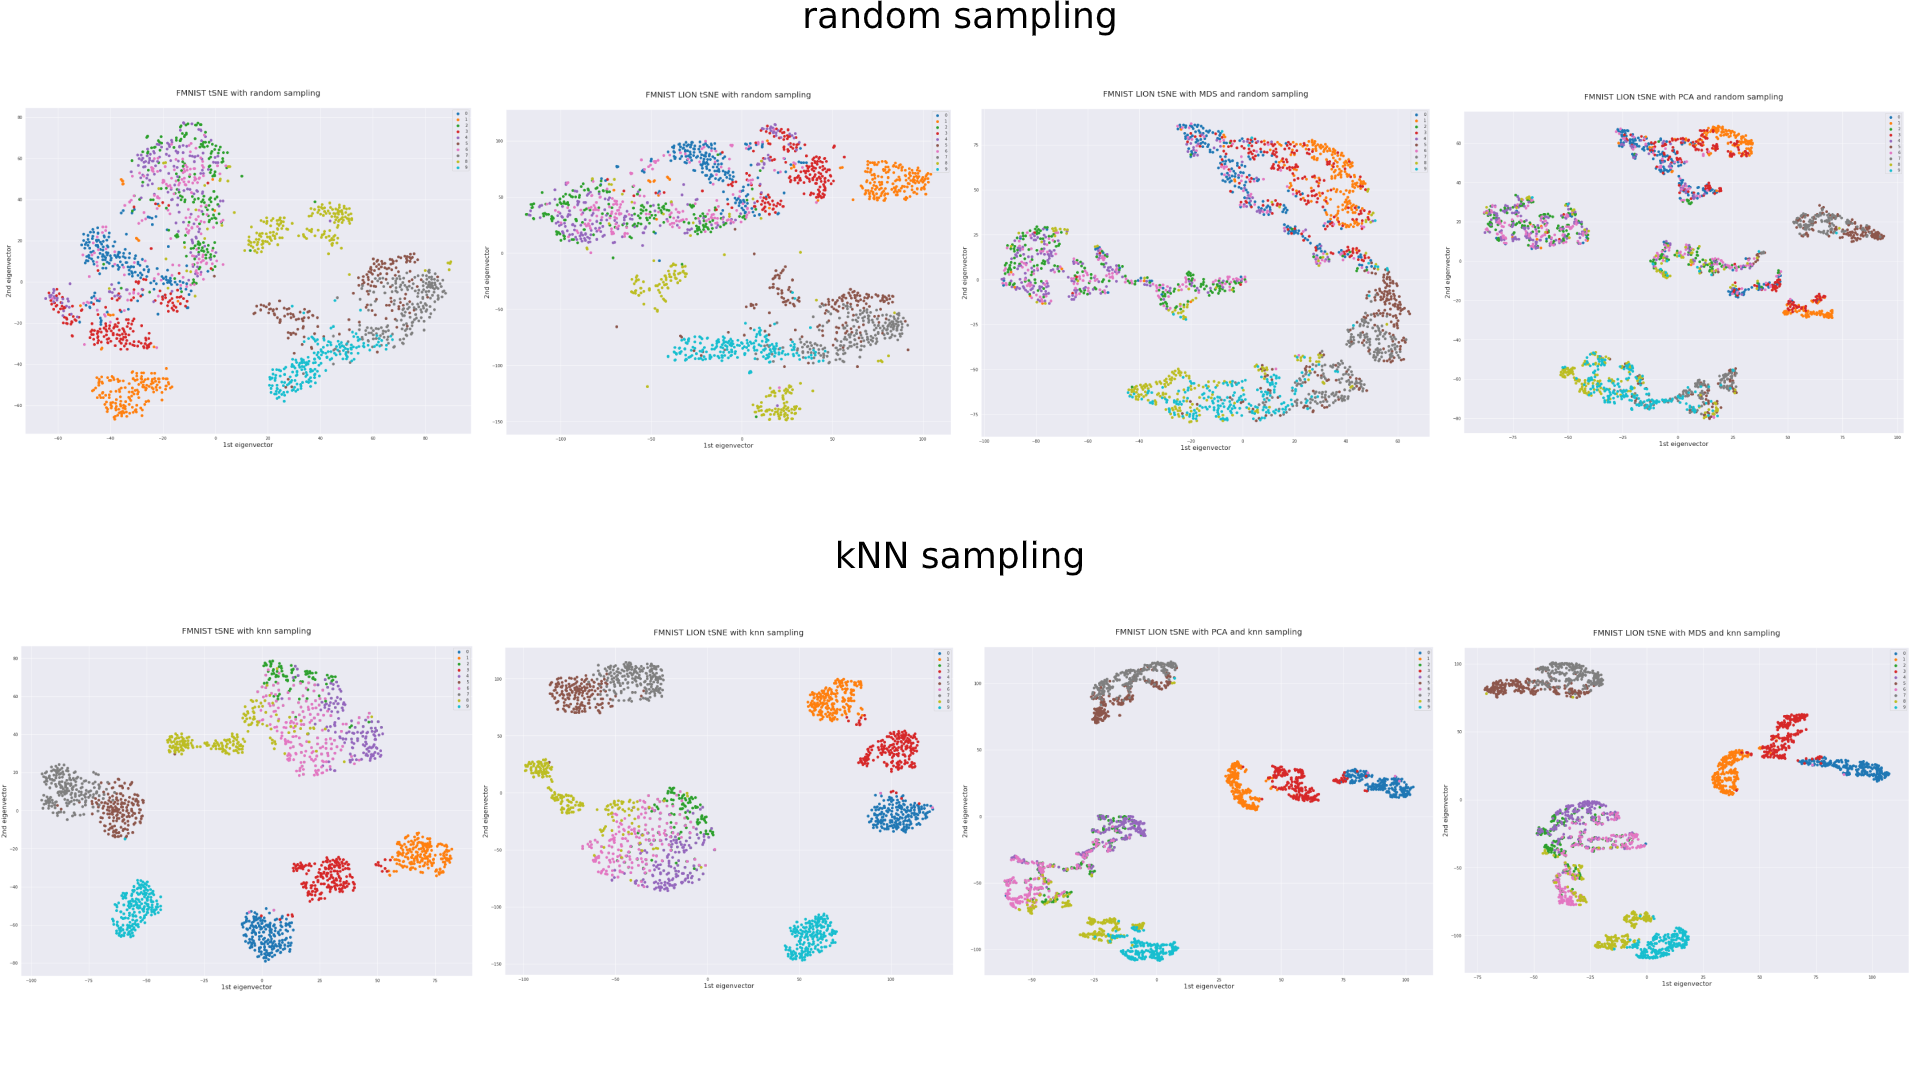
\includegraphics[scale=0.25]{fmnist-dataset-results.png}
\caption{Wizualizacja Fashion MNIST Dataset za pomocą różnych metod}
\end{figure}

    \item Reuters Dataset \cite{reuters-dataset}
\paragraph{}
Dataset stworzony z dokumentów pochodzącejz kolekcji Reuters-21578, która ukazała się w głównym kanale publikacji agencji Reuters w 1987. Dokumenty zostały złożone i zindeksowane na kategorię przez personel agencji Reuters Ltd. (Sam Dobbins, Mike Topliss, Steve Weinstein) oraz Carnegie Group, Inc. (Peggy Andersen, Monica Cellio, Phil Hayes, Laura Knecht, Irene Nirenburg) w 1987.

W 1990 dokumenty zostały opublikowane przez Reuters i CGI do celów badawczych dla Information Retrieval Laboratory (W. Bruce Croft, Director) z wydziału Informatyki Uniwersytetu Massachusetts w Amherst. Formatowanie dokumentów i stworzenie zwiuązanych z tym plików zostało wykonane w 1990 przez Davida D. Lewisa and Stephena Hardinga z Information Retrieval Laboratory.

\begin{figure}[h]
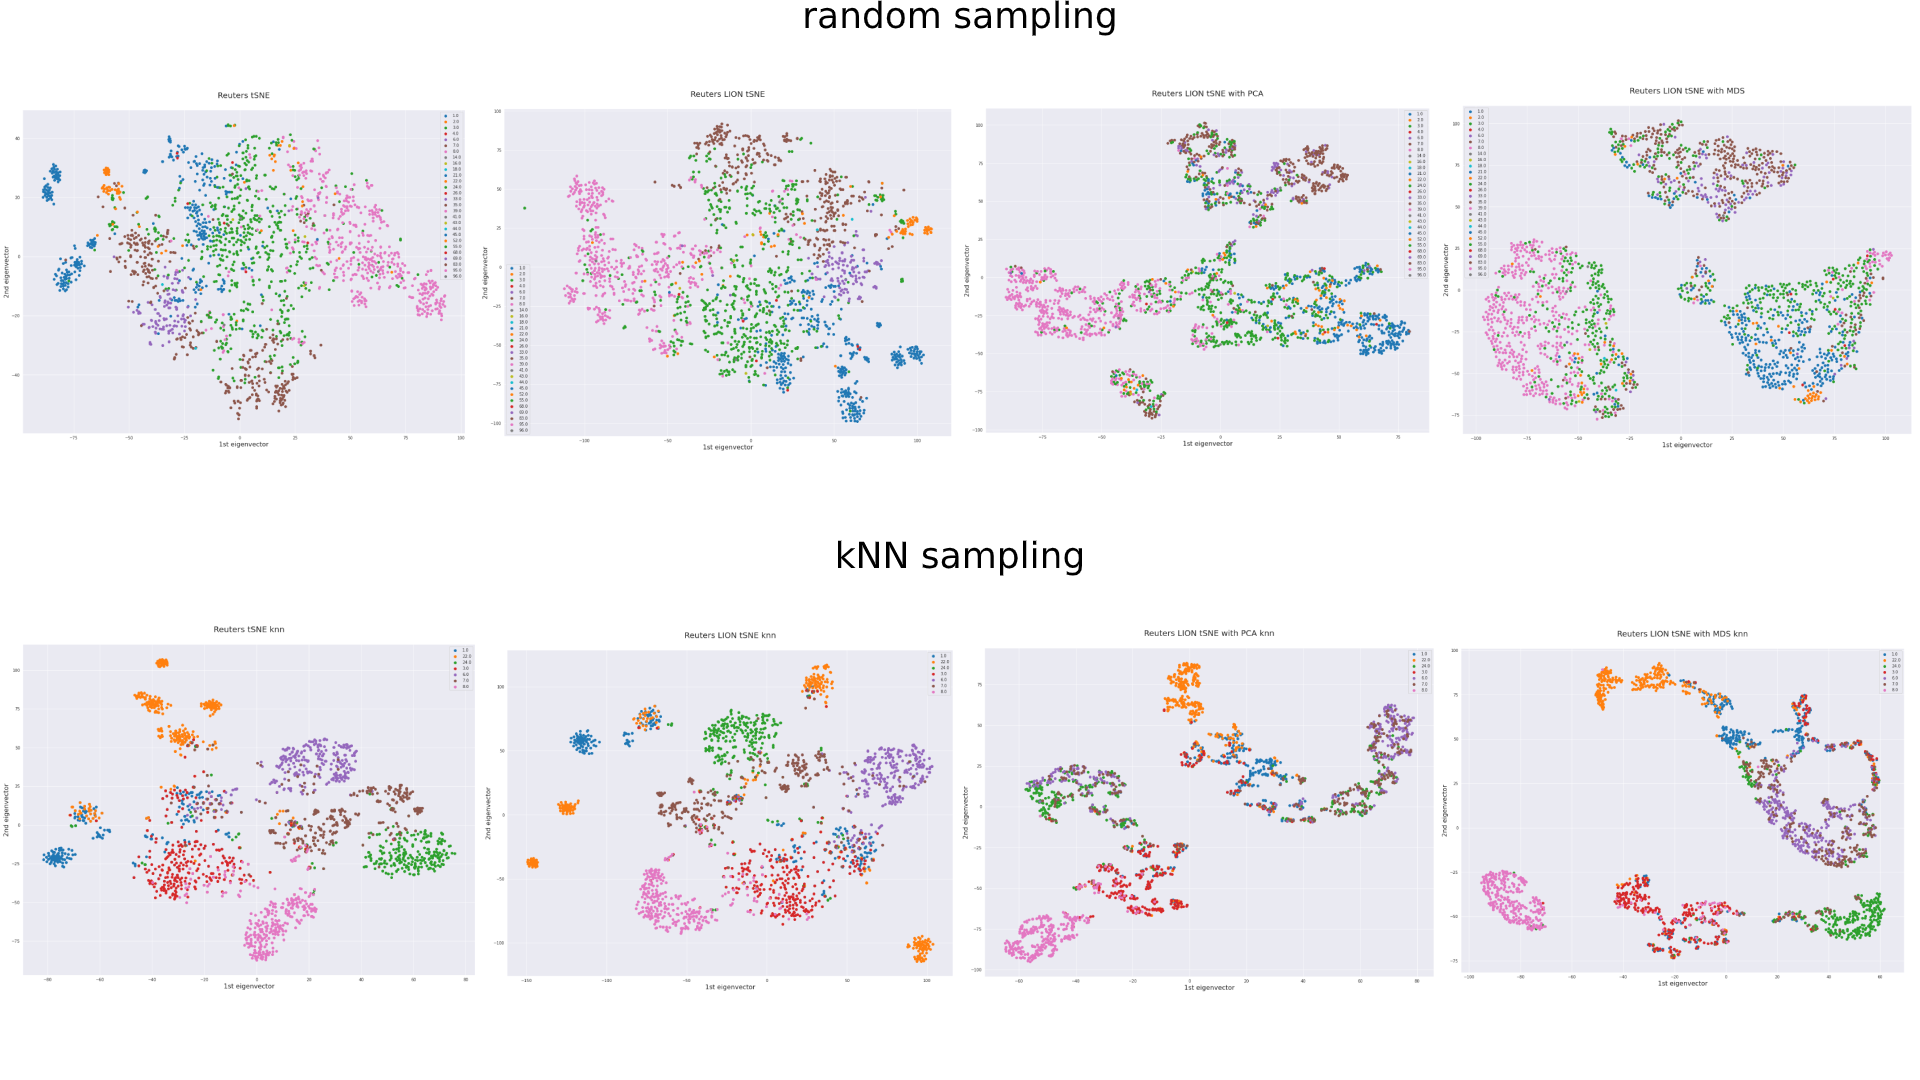
\includegraphics[scale=0.25]{reuters-dataset-results.png}
\caption{Wizualizacja Reuters Dataset za pomocą różnych metod}
\end{figure}

\end{itemize}

\subsection{Wykorzystane metryki}
TODO
 
\section{Wnioski}
\label{sec:conclusions}
TODO

\bibliographystyle{unsrt}  
%\bibliography{references}  %%% Remove comment to use the external .bib file (using bibtex).
%%% and comment out the ``thebibliography'' section.


%%% Comment out this section when you \bibliography{references} is enabled.
\clearpage
\renewcommand\refname{Źródła}
\begin{thebibliography}{1}

\bibitem{paper} 
Bheekya Dharamsotu ; K. Swarupa Rani ; Salman Abdul Moiz ; C. Raghavendra Rao
\newblock Paper: k-NN Sampling for Visualization of Dynamic Data Using LION-tSNE. 
\newblock {\em https://ieeexplore.ieee.org/abstract/document/8990391}

\bibitem{tsne-paper} 
Laurens van der Maaten ; Geoffrey Hinton
\newblock Paper: Visualizing Data using t-SNE 
\newblock {\em http://www.cs.toronto.edu/~hinton/absps/tsne.pdf}


\bibitem{lion-paper} 
Andrey Boytsov ; François Fouquet ; Yves Le Traon
\newblock Paper: Visualizing and Exploring Dynamic High-Dimensional Datasets with LION-tSNE. 
\newblock {\em https://github.com/andreyboytsov/LION-tSNE}

\bibitem{lion-github} 
Andrey Boytsov
\newblock LION tSNE Github Repository. 
\newblock {\em https://github.com/andreyboytsov/LION-tSNE}

\bibitem{iris-dataset} 
\newblock IRIS Dataset. 
\newblock {\em https://archive.ics.uci.edu/ml/datasets/iris}

\bibitem{mnist-dataset} 
\newblock MNIST Dataset. 
\newblock {\em http://yann.lecun.com/exdb/mnist/}

\bibitem{fmnist-dataset} 
\newblock FASHION MNIST Dataset. 
\newblock {\em https://research.zalando.com/welcome/mission/research-projects/fashion-mnist/}

\bibitem{reuters-dataset} 
\newblock REUTERS Dataset. 
\newblock {\em https://archive.ics.uci.edu/ml/datasets/Reuters-21578+Text+Categorization+Collection}

\end{thebibliography}



\end{document}

